% Number 40
% Algebra
% Quartic equation solving algebra problem
% MIT Physics for Teachers LON-CAPA

% Watermark
\AddToShipoutPicture*{\BackgroundPic}

\addtocounter {ProbNum} {1}

%\begin{floatingfigure}[r]{.2\textwidth}
%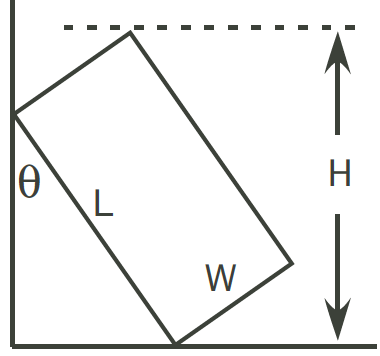
\includegraphics[scale=1]{/Users/jgates/desktop/latex/pics/leaningbox.png}
%\end{floatingfigure}
 
{\bf \Large{\arabic{ProbNum}}} Find all possible values of $x$ which solve the equation ${x^{4}-20\cdot x^{2}+64=0}$.

%\bigskip

%\indent How many nickels and how many dimes does she have? 

\vfill

\newpage
